\SourcePage{656}{661}
\setcounter{chapter}{12}
\chapter{Asymptotic Formulae of Quantum Electrodynamics}
\setcounter{section}{131}
\section{High-Momentum Asymptotics of the Photon Propagator}

In \S~113 we calculated the first term (in $\alpha$) in the expansion of the polarization operator $\mathcal P(k^2)$. To logarithmic accuracy, its form for $|k^2|\gg m^2$ was found to be
\begin{equation}
\mathcal P(k^2)=\frac{\alpha}{3\pi}k^2\ln\frac{|k^2|}{m^2}.
\tag{132.1}
\end{equation}
It was also noted there that the derivation of this formula, as a first-order correction to the propagator $4\pi D^{-1}=k^2$, presupposes the condition
\begin{equation}
\frac{\alpha}{3\pi}\ln\frac{|k^2|}{m^2}\ll 1.
\tag{132.2}
\end{equation}
This limits its range of applicability at large $|k^2|$. We shall now show that (132.1) in fact remains valid under the much weaker condition
\begin{equation}
\frac{\alpha}{3\pi}\ln\frac{|k^2|}{m^2}\lesssim 1.
\tag{132.3}
\end{equation}

The argument proceeds as follows.\footnote{This formulation of the problem and the results presented here are due to L.~D.~Landau, A.~A.~Abrikosov, and I.~M.~Khalatnikov (1954).} First observe that, although terms of every order in $\alpha$ in the perturbation series can in principle contribute to $\mathcal P(k^2)$ under condition (132.3), at order $n$ it is enough to retain only terms $\sim\alpha^n\ln^n(|k^2|/m^2)$, in which the large logarithm has the same power as $\alpha$. Terms containing lower powers of the logarithm are necessarily small because $\alpha\ll1$.

The perturbation series for $\mathcal P$ can next be reduced to those for $G$ and $\Gamma^\mu$ by means of the Dyson equation
\begin{equation}
\mathcal P(k^2)=i\frac{4\pi\alpha}{3}\Tr\int\gamma_\mu G(p+k)\Gamma^\mu(p+k,p;k)G(p)\frac{d^4p}{(2\pi)^4}
\tag{132.4}
\end{equation}
\SourcePage{657}{662}
(see (107.4)). Since $\mathcal P(k^2)$ is gauge invariant, any gauge may be chosen for $G$ and $\Gamma$. The Landau gauge is especially convenient here; in this gauge the free-photon propagator has the form (76.11)
\begin{equation}
D_{\mu\nu}(k)=\frac{4\pi}{k^2}\left(g_{\mu\nu}-\frac{k_\mu k_\nu}{k^2}\right)
\tag{132.5}
\end{equation}
($D^{(l)}=0$ in (103.17)). It turns out that, in this gauge, the perturbation expansions of $G$ and $\Gamma^\mu$ contain no terms with the required powers of the logarithms. Thus their zeroth-order values, $G=G_0$ and $\Gamma^\mu=\gamma^\mu$, suffice in (132.4), which then becomes
\begin{equation}
\mathcal P(k^2)=i\frac{4\pi\alpha}{3}\Tr\int\gamma_\mu G(p+k)\gamma^\mu G(p)\frac{d^4p}{(2\pi)^4}.
\tag{132.6}
\end{equation}
This is the Feynman integral represented by the first-order (in $\alpha$) diagram (113.1), and, after the appropriate renormalization, it gives (132.1).

To prove these statements, let us first trace the origin of the logarithm in (132.6). The logarithmic term plainly comes from the integration region
\begin{equation}
p^2\gg|k^2|\quad\text{when}\quad |k^2|\gg m^2.
\tag{132.7}
\end{equation}
Indeed, a formal expansion of $G$ in powers of $1/(\gamma p)$ gives
\[
G(p)\approx\frac{1}{\gamma p}=\frac{\gamma p}{p^2},
\]
\[
\begin{aligned}
G(p-k)&\approx\frac{1}{\gamma p-\gamma k}\approx
\frac{1}{\gamma p}+\frac{1}{\gamma p}\gamma k\frac{1}{\gamma p}
+\frac{1}{\gamma p}\gamma k\frac{1}{\gamma p}\gamma k\frac{1}{\gamma p}=\\
&=\frac{\gamma p}{p^2}+\frac{(\gamma p)(\gamma k)(\gamma p)}{(p^2)^2}
+\frac{(\gamma p)(\gamma k)(\gamma p)(\gamma k)(\gamma p)}{(p^2)^3}.
\end{aligned}
\]
On substitution in (132.6), the first term, which is independent of $k$, is removed by regularization, consistently with the requirement $\mathcal P/k^2\to0$ as $k^2\to0$. The second term vanishes upon angular integration over $p$. The integral from the third term, however, diverges logarithmically in $p^2$. Taking its limits from $p^2\sim|k^2|$, the lower boundary of region (132.7), to an auxiliary ``cutoff parameter'' $\Lambda^2$, we obtain
\begin{equation}
-\frac{\alpha}{3\pi}k^2\ln\frac{\Lambda^2}{|k^2|}.
\tag{132.8}
\end{equation}
Regularization requires subtracting from $\mathcal P/k^2$ its value at $k^2=0$. Logarithmic accuracy, however, assumes
\SourcePage{658}{663}
$|k^2|\gg m^2$, so to this accuracy regularization amounts to subtracting the value at $|k^2|\sim m^2$. Consequently $\Lambda^2$ in the logarithm is replaced by $m^2$, and (132.1) follows.

The corrections of interest in $G$ and $\Gamma^\mu$ are logarithmic. When these are included, the exact functions therefore differ from $G_0$ and $\gamma^\mu$ only by slowly varying logarithmic factors. The same region (132.7) that matters in the approximate integral (132.6) is accordingly important in the exact integral (132.4). Nevertheless, one cannot simply set $k=0$ in $\Gamma^\mu(p+k,p;k)$: because the integral is quadratically divergent, its regularization also requires the next two terms in the expansion of $\Gamma^\mu(p+k,p;k)$ in powers of $k$. Here, however, we shall discuss only the corrections to $\Gamma^\mu(p,p,0)$. This already shows clearly both why the choice of gauge matters and how the integrals associated with diagrams of different types differ. There is no need to carry out an analogous investigation of $G$, since the corrections to $\Gamma$ and $G$ are related by the Ward identity (108.8).

The first-order correction (in $\alpha$) to $\Gamma(p,p;0)$ corresponds to the diagram
\begin{center}
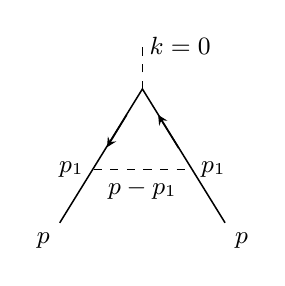
\begin{tikzpicture}[x=1cm,y=1cm,>=stealth,line width=.55pt,font=\small]
  \coordinate (t) at (0,1.65);
  \coordinate (l) at (-.62,.63);
  \coordinate (r) at (.62,.63);
  \coordinate (bl) at (-1.05,-.05);
  \coordinate (br) at (1.05,-.05);
  \draw (bl)--(t)--(br);
  \draw[dashed] (l)--(r);
  \draw[dashed] (t)--(0,2.28);
  \draw[->] (-.20,1.32)--(-.45,.91);
  \draw[->] (.46,.90)--(.20,1.32);
  \node[above right=-1pt] at (0,2.00) {$k=0$};
  \node[left] at (l) {$p_1$};
  \node[right] at (r) {$p_1$};
  \node[below] at (0,.63) {$p-p_1$};
  \node[below left] at (bl) {$p$};
  \node[below right] at (br) {$p$};
\end{tikzpicture}
\end{center}
and hence to the integral\footnote{To avoid confusion in comparing with the results of \S~117, recall that in \S~117 both electron ends of the diagram were taken to be physical. Here, by contrast, $p^2\gg|k^2|\gg m^2$, so neither line is physical.}
\begin{equation}
\Gamma^{\mu(1)}=-i\alpha\int\gamma^\lambda G(p_1)\gamma^\mu G(p_1)\gamma^\nu D_{\lambda\nu}(p-p_1)\frac{d^4p_1}{(2\pi)^4}.
\tag{132.9}
\end{equation}
In the usual gauge,
\[
D_{\lambda\nu}(p-p_1)=g_{\lambda\nu}\frac{4\pi}{(p-p_1)^2},
\]
and the relevant integration region is $p_1^2\gg p^2$, where the integral diverges logarithmically. Evaluating
\begin{equation}
\Gamma^{\mu(1)}\approx-4\pi i\alpha\int
\frac{\gamma^\lambda(\gamma p_1)\gamma^\mu(\gamma p_1)\gamma_\lambda}{(p_1^2)^3}
\frac{d^4p_1}{(2\pi)^4}
\tag{132.10}
\end{equation}
\SourcePage{659}{664}
and regularizing the logarithm gives
\[
\Gamma^{\mu(1)}\approx-\frac{\alpha}{4\pi}\gamma^\mu\ln\frac{p^2}{m^2}.
\]
In the Landau gauge, on the other hand, (132.10) is replaced by
\[
\Gamma^{\mu(1)}\approx-4\pi\alpha i\int
\left\{\gamma^\lambda(\gamma p_1)\gamma^\mu(\gamma p_1)\gamma_\lambda-p_1^2\gamma^\mu\right\}
\frac{d^4p_1}{(p_1^2)^3(2\pi)^4}.
\]
After averaging over the directions of $p_1$ and reducing the $\gamma$ matrices, this integral is zero; the logarithmic term in $\Gamma^{\mu(1)}$ therefore disappears.\footnote{The corrections to $G^{-1}$ in the two gauges, obtained from the correction $\Gamma^{(1)}$ by means of identity (108.8), agree, of course, with the results of \S~119.}

Among the second-order corrections (in $\alpha$), consider the diagram
\begin{center}
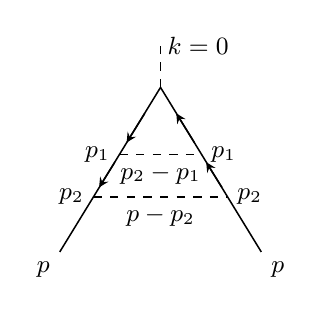
\begin{tikzpicture}[x=1cm,y=1cm,>=stealth,line width=.55pt,font=\small]
  \coordinate (t) at (0,2.15);
  \coordinate (l1) at (-.52,1.30);
  \coordinate (r1) at (.52,1.30);
  \coordinate (l2) at (-.85,.76);
  \coordinate (r2) at (.85,.76);
  \coordinate (bl) at (-1.28,.06);
  \coordinate (br) at (1.28,.06);
  \draw (bl)--(t)--(br);
  \draw[dashed] (l1)--(r1);
  \draw[dashed] (l2)--(r2);
  \draw[dashed] (t)--(0,2.75);
  \draw[->] (-.20,1.82)--(-.43,1.45);
  \draw[->] (-.58,1.20)--(-.78,.88);
  \draw[->] (.78,.88)--(.58,1.20);
  \draw[->] (.43,1.45)--(.20,1.82);
  \node[above right=-1pt] at (0,2.48) {$k=0$};
  \node[left] at (l1) {$p_1$};
  \node[right] at (r1) {$p_1$};
  \node[left] at (l2) {$p_2$};
  \node[right] at (r2) {$p_2$};
  \node[below] at (0,1.30) {$p_2-p_1$};
  \node[below] at (0,.76) {$p-p_2$};
  \node[below left] at (bl) {$p$};
  \node[below right] at (br) {$p$};
\end{tikzpicture}
\end{center}
The corresponding integral is
\[
\begin{aligned}
\Gamma^{\mu(2)}={}&-\alpha^2\int
\gamma^\lambda G(p_2)\gamma^\nu G(p_1)\gamma^\mu G(p_1)\gamma^\rho G(p_2)\gamma^\sigma\,\times\\
&\times D_{\nu\rho}(p_2-p_1)D_{\lambda\sigma}(p-p_2)
\frac{d^4p_1\,d^4p_2}{(2\pi)^8}.
\end{aligned}
\]
With the usual gauge for the $D$ functions, this integral contains a squared-logarithm term arising from the region
\begin{equation}
p_1^2\gg p_2^2\gg p^2.
\tag{132.11}
\end{equation}
Indeed, after $p_2$ is neglected in the argument of $D_{\nu\rho}(p_2-p_1)$, the integration over $d^4p_1$ is of the same kind as in (132.9) and yields $\ln p_2^2$. The subsequent integration over $d^4p_2$ is logarithmic once again and produces the square of $\ln(p^2/m^2)$. If the Landau gauge is used for the $D$ functions, however, the logarithmic terms vanish in both integrations.

\SourcePage{660}{665}
The same holds for every other diagram belonging to the skeleton diagram
\begin{equation}
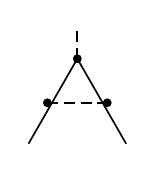
\begin{tikzpicture}[baseline=-.45ex,x=1cm,y=1cm,line width=.6pt]
  \coordinate (t) at (0,.80);
  \coordinate (l) at (-.38,.24);
  \coordinate (r) at (.38,.24);
  \draw (-.62,-.28)--(t)--(.62,-.28);
  \draw[line width=.8pt,dash pattern=on 4pt off 2pt] (t)--(0,1.18);
  \draw[line width=.8pt,dash pattern=on 4pt off 2pt] (l)--(r);
  \fill (t) circle (1.6pt) (l) circle (1.6pt) (r) circle (1.6pt);
\end{tikzpicture}
\tag{132.12}
\end{equation}
Diagrams of other types, with crossing photon lines, such as those contained in the skeleton diagram
\begin{equation}
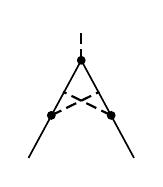
\begin{tikzpicture}[baseline=-.45ex,x=1cm,y=1cm,line width=.6pt]
  \coordinate (t) at (0,.88);
  \coordinate (l) at (-.38,.18);
  \coordinate (r) at (.38,.18);
  \draw (-.67,-.36)--(t)--(.67,-.36);
  \draw[line width=.8pt,dash pattern=on 4pt off 2pt] (t)--(0,1.28);
  \draw[line width=.8pt,dash pattern=on 4pt off 2pt] (l)--(.23,.48);
  \draw[line width=.8pt,dash pattern=on 4pt off 2pt] (r)--(-.23,.48);
  \fill (t) circle (1.6pt) (l) circle (1.6pt) (r) circle (1.6pt);
\end{tikzpicture}
\tag{132.13}
\end{equation}
(cf. (106.11)), contain no terms with the required power of the logarithm in any gauge. For these diagrams there is no region of the integration variables in which the integral can be reduced to a succession of logarithmic integrations.

These arguments, together with their analogues for the following terms in the expansion of $\Gamma$ in powers of $k$, confirm that in the Landau gauge no corrections to $G$ and $\Gamma$ arise with the required powers of the logarithm. Expression (132.1) is therefore valid under condition (132.3) as asserted.

The function $D(k^2)$ corresponding to the polarization operator (132.1) is
\begin{equation}
D(k^2)=\frac{4\pi}{k^2}\,
\frac{1}{1-\dfrac{\alpha}{3\pi}\ln\dfrac{|k^2|}{m^2}}.
\tag{132.14}
\end{equation}
Under condition (132.3), there is no need to expand this expression in powers of $\alpha$.
